\subsection{トルクと粒子の回転}
\label{sec:rotation}
せん断流下に球形粒子が存在する場合,流体から受けるトルクは式\eqref{eq:hydro_torque}で表される.

    \begin{equation}
        \boldsymbol{N}^\mathrm{H} = 4 \pi \mu a^3 \dot{\gamma}
        \label{eq:hydro_torque}
    \end{equation}

\noindent
ここで,$\mu$は流体の粘度,$a$は粒子の半径,$\dot{\gamma}$はせん断速度である.
流体から受けるトルクに加えて,\ref{sec:equation_of_motion}で述べたbottom heavy性によるトルクを考えることで,粒子の回転の有無を考えることができる.
せん断速度が小さい場合には,bottom heavy性によるトルクが支配的となり,トルクの和が0となる角度で粒子の進行方向が固定され,回転しないことが予想される.
一方,せん断速度が大きい場合には,流体から受けるトルクが支配的となり,粒子が定常的に回転することが予想される.
このように,流体から受けるトルクとbottom heavy性によるトルクの釣り合いから,粒子の進行方向が異方的になることが予想される.

\begin{figure}[htbp]
    \centering
    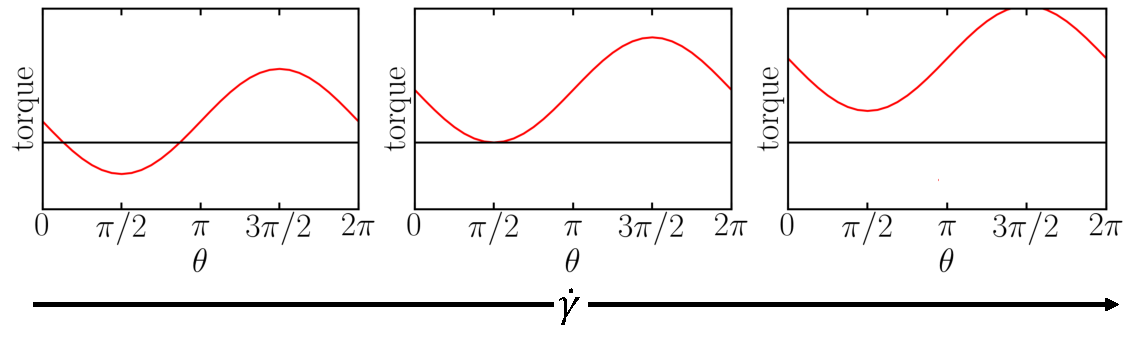
\includegraphics[scale=0.8]{/Users/taiga/Projects/lab/thesis/components/chapter3/figs/sum_torque.pdf}
    \caption{流体から受けるトルクとbottom heavy性によるトルクの和とせん断速度との関係}
    \label{eq:sum_torque}
\end{figure}
